\documentclass[12pt, logo=tehranDLDL/ut]{tehranDLDL}
\usepackage{pgfplots}
\usepackage[american, siunitx]{circuitikz}
\usepackage{tikz-timing}
\usepackage{subcaption}

\suptitle{}
\supsubtitle{}
\title{Lab Manual}
\author{Hadi Safari}
\preparer{\href{mailto:hadi.safari@ut.ac.ir?subject=[DLDLab]\%20}{Hadi Safari}}
\supervisor{Professor Z. Navabi}
\university{University of Tehran}
\college{College of Engineering\\School of Electrical \& Computer Engineering}
\course[DLLab]{Digital Logic Laboratory}
\coursecode{ECE 045}
\courseurl{https://cecm.ut.ac.ir/course/view.php?id=2702}
\date{Spring 1398}

\graphicspath{{img/manual/}}
\usetikzlibrary{positioning, shapes.multipart}

\begin{document}

\maketitle

\tableofcontents
\newpage

\section*{Introduction}
\addcontentsline{toc}{section}{Introduction}

This manual is prepared to help you get familiar with devices, tools, and equipment of the \textsc{Digital Logic Laboratory}. In addition, it will help you with the proper procedure of debugging analog and digital circuits. Please have this manual with yourselves in every session of the course.

\section{Breadboard}

A breadboard is a simple construction which is commonly used for prototyping electronic circuits. These boards have two parts that their connection is different from each other. \Fref{fig:breadboard} shows a simple breadboard.

\begin{figure}[b]
    \centering
    \caption{A simple breadboard and its connections\label{fig:breadboard}}
    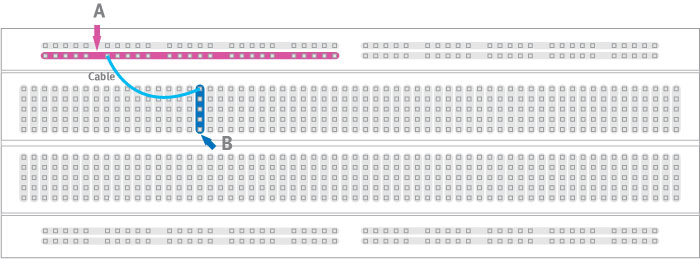
\includegraphics[width=0.8\textwidth]{breadboard.jpg}
\end{figure}

\Fref{fig:breadboard} shows one possible connection pattern of a breadboard. The outer parts of the breadboards are connected horizontally (Part A) and the inner parts are connected vertically (Part B). It is important to note that in some breadboards, such as \fref{fig:breadboard}, all of the two lines in Part A are not connected together and if a large circuit is implemented on a breadboard, you need to connect the two sides using wires. On the other hand, there are some breadboards, such as \fref{fig:connected-breadboard}, which do not follow the same pattern for the mentioned part and they usually have blue and red lines to indicate their connection pattern.

\begin{figure}
    \centering
    \caption{Another connection pattern of breadboards\label{fig:connected-breadboard}}
    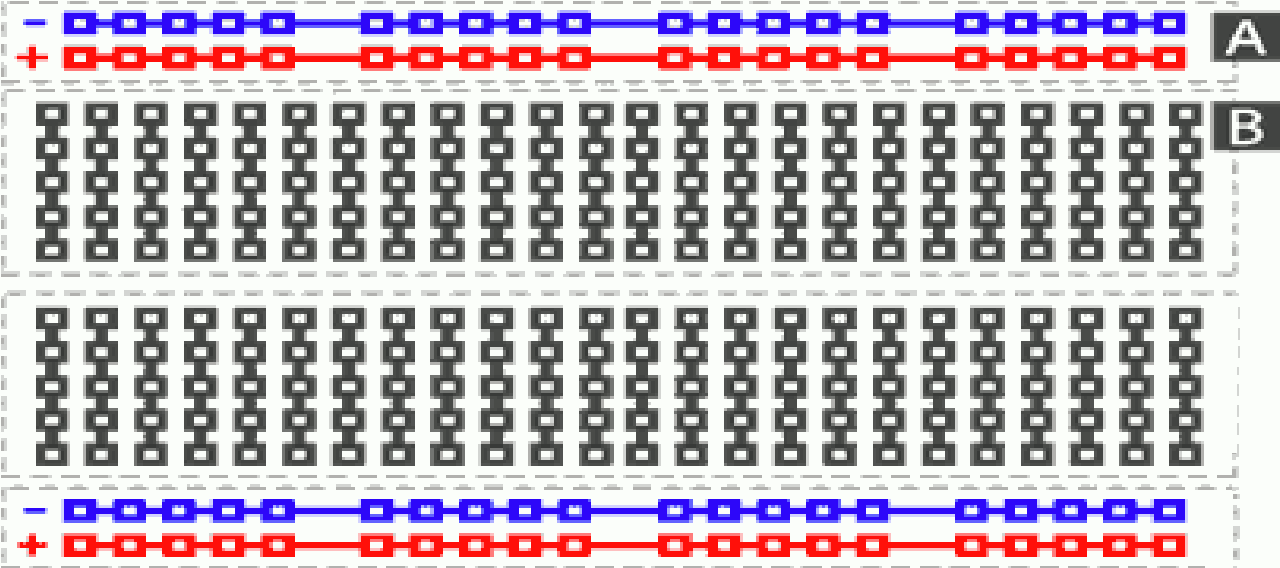
\includegraphics[width=0.5\textwidth]{breadboard.png}
\end{figure}

The outer part of the breadboards, here Part A, is mainly designed for supply and ground voltages in order to isolate these voltages from other parts of a design and also organize the circuit.

In all breadboards, there is a deep line in the middle of the board which is called \textit{ravine}. This ravine serves a very important purpose. Many integrated circuits---often referred to as ICs or, simply, chips---are manufactured specifically to fit onto breadboards. In order to minimize the amount of space they take up on the breadboard, they come in what is known as a Dual in-line Package, or DIP.

\begin{figure}
    \centering
    \caption{Ravine for ICs\label{fig:ravine}}
    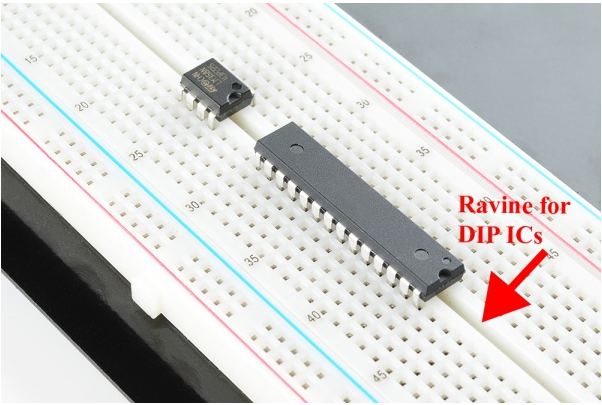
\includegraphics[width=0.4\textwidth]{ravine.png}
\end{figure}

These DIP chips have legs that come out of both sides and fit perfectly over that ravine. Since each leg on the IC is unique, we don't want both sides to be connected to each other. That is where the separation in the middle of the board comes in handy. Thus, we can connect components to each side of the IC without interfering with the functionality of the leg on the opposite side.

\section{Building and Debugging a Circuit on a Breadboard}

In this lab, there are some parts of the circuits that are designed outside of FPGA and they are implemented on your breadboards. Following these steps will help you debug your circuit more conveniently and less time-consuming. 

\subsection{Building the Circuit\label{sec:building-circuit}}

\paragraph*{Important}
Before connecting anything to a circuit, always verify the power supply voltages and input signals with an oscilloscope or voltmeter. Even if the instrument display seems to indicate levels are correct, this is a good practice to prevent circuit or equipment damage.

\begin{enumerate}
    \item Wire power and ground neatly and carefully around the perimeter of breadboards. Stick to a convention (for example, use red wires for $V_\mathit{DD}$, and black wires for $\mathit{GND}$) to facilitate debug and help prevent damaging equipment or components. Pay attention to which sections of the breadboard are permanently shorted together and which sections are not.
    \item Have the design complete prior to building the circuit. This includes a \textit{floor plan}, showing the relative placement of chips on your breadboard, and a diagram showing how every pin is connected. This will help with having a neat and clean design which makes debugging far easier. You will likely spend less total time on your project if you do this first.
    \begin{figure}
        \centering
        \caption{An example of floor plan\label{fig:floorplan}}
        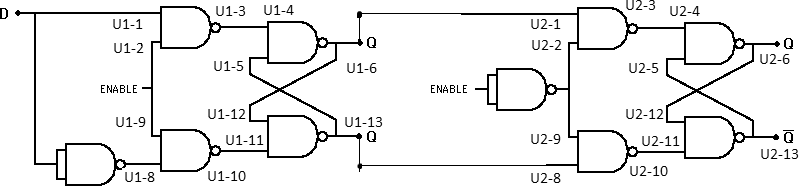
\includegraphics[width=0.7\textwidth]{floorplan.png}
    \end{figure}
    \item Place all necessary ICs in the breadboard paying attention to where signals will be routed around the board. Try to avoid long wires; they can be messy and can potentially cause operational problems and induce more interference into circuits.
    \item Before starting to wire, keep in mind that long looping wires make it harder to debug and can induce unwanted interference into the circuit. It is a good idea to check the connectivity of the two ends of the wires by using digital multimeters in order to avoid any unwanted disconnection. 
    \item Next, wire up power and ground to all the ICs, stick with the same convention chosen above to keep things organized.
    \item Then wire in all static signals (i.e.\ signals that will be wired directly to power or ground). These may be enable signals or a load signals.
    \item Wire the remainder of the circuit trying to be as neat as possible. Remember, some extra time up front can save you from some serious headaches when debugging later on.
    \item If possible, it is often helpful to check circuit functionality as you build. Build a small sub-circuit, then test its result before moving on to another sub-circuit.
\end{enumerate}

\subsection{Debugging the Circuit}

\begin{enumerate}
    \item As noted in \fref{sec:building-circuit}, it is often helpful to test as you build, by building sub-circuits and then testing those intermediate results before moving onto the next sub-circuit.
    \item Start by checking part numbers on the ICs to verify that they are indeed the desired component.
    \item Next, check the power and ground pins of all ICs. Focus especially on those in the area where the problem seems to be occurring.
    \item Check that enable and/or clear type signals are properly set.
    \item Check that all inputs to all the gates being used in the circuit are connected to valid logic signals (i.e.\ power, ground or signal). Even if the pin is not needed for the particular implementation, if it is left unconnected the circuit will often not function properly and have odd results. For example, if a 3-input AND gate is needed for the design, but a 4-input AND gate is all that is available in the circuit, the fourth input should be tied to $V_\mathit{DD}$, also called $V_\mathit{CC}$.
    \item For clocked circuits or circuits with external inputs, recheck the input signal directly from the function generator or module. This should have been done once already before applying the signal to the circuit.
    \item Start with the outputs. Check if the output is justified with its inputs according to the logic gate or digital circuit functionality. If the output is correct, move on to the previous output and one step closer to the input. Continue this procedure until you find the faulty output. If the output is not justified with the inputs of the circuit, there are several possible problems:
    \begin{enumerate}
        \item First cause could be a fault in supply voltages. Please check if all the ICs are properly connected to ground and $V_\mathit{DD}$. 
        \item Second cause could be a short between two lines. If there is an intermediate voltage (i.e.\ \SI{2}{\volt} or \SI{2}{\volt}) on a pin, there may be a short between two nodes (i.e.\ two pins with different logic values are connected unintentionally).
        \item Another cause might be that the IC is faulty. In this case try the circuit with another IC. 
        \item Another possibility could be the springs on the breadboards or the wires that are making unwanted connections or contentions.
    \end{enumerate}
    Of course, there is a long list of other hardware issues that must be detected during the procedure of debugging. 
    \item Continue moving towards the input and try to isolate problems.
    \item Often adding intermediate results (i.e.\ additional LEDs or indicators) helps to isolate problems, especially in large circuits.
\end{enumerate}

\section{Oscilloscope Guide}

The main purpose of an oscilloscope is to graph an electrical signal as it varies over time. Most scopes produce a two-dimensional graph with time on the x-axis and voltage on the y-axis. 

Many scopes have measurement tools, which help to quickly quantify frequency, amplitude, and other waveform characteristics. In general, a scope can measure both time-based and voltage-based characteristics:

\begin{description}[font=\labelitemi\ \bfseries]
    \item[Timing characteristics]~
    \begin{description}[font=\labelitemii\ \bfseries]
        \item[Frequency \& period]
        Frequency is defined as the number of times per second a waveform repeats.
        Period is the reciprocal of that, i.e.\ number of seconds each repeating waveform takes.\\
        The maximum frequency a scope can measure varies, but it is often in the 100's of \SI{}{\mega\hertz} (1E6~\SI{}{\hertz}) range.
        \item[Duty cycle]
        The percentage of a period that a wave is either positive or negative (there are both positive and negative duty cycles).\\
        The duty cycle is a ratio that tells you how long a signal is \textit{on} versus how long it's \textit{off} each period.
        \item[Rise \& fall time]
        Signals can't instantaneously go from \SI{0}{\volt} to \SI{5}{\volt}. They have to smoothly rise. The duration of a wave going from a low point to a high point is called the rise time, and fall time measures the opposite.\\
        These characteristics are important when considering how fast a circuit can respond to signals.
    \end{description}
    \item[Voltage characteristics]~
    \begin{description}[font=\labelitemii\ \bfseries]
        \item[Amplitude]
        Amplitude is a measure of the magnitude of a signal.\\
        There are a variety of amplitude measurements including peak-to-peak and peak amplitude.
        Peak-to-peak which measures the absolute difference between a high and low voltage point of a signal.
        Peak amplitude, on the other hand, only measures how high or low a signal is over \SI{0}{\volt}.
        \item[Maximum \& minimum voltages]
        The scope can tell you exactly how high and low the voltage of your signal gets.
    \end{description}
\end{description}

Oscilloscopes come in two varieties: analog and digital. The controls on both types are basically the same.
Be aware that the digital scopes may hide some of their controls in a menu on the LCD display instead of using knob or button.

All oscilloscopes have some basic controls in common.
Be sure you can identify these controls on your oscilloscope:
\begin{description}[font=\labelitemi\ \bfseries]
    \item[Probe input] At least one input where an oscilloscope probe (also called a coaxial cable) can be attached\\
    Be sure you have one of these cables.
    \item[Screen with a grid overlay]
    This grid is useful when you want to make measurements using the scope.
    \item[Volts/div]
    This control lets you change how many volts are represented by each vertical increment of grid overlay on the screen. Basically, it allows you to zoom in and out along the y-axis.
    \item[Time/div]
    This control lets you change how much time is represented by each horizontal increment of the grid overlay on the screen. It allows you to zoom in and out along the x-axis.
    \item[Vertical position/offset]
    Lets you move up and down in the y direction.
    \item[Horizontal position/offset]
    Move left and right.
    \item[Trigger level]
    This is a tool that allows you to stabilize your waveform on the screen.
\end{description}

\subsection{Vertical System}

The \textbf{vertical} section of the scope controls the \textbf{voltage scale} on the display. There are traditionally two knobs in this section, which allow you to individually control the vertical position and volts/div.

The more critical \textbf{volts per division (volts/div)} knob allows you to set the vertical scale on the screen. Rotating the knob clockwise will decrease the scale, and counter-clockwise will increase. A smaller scale (fewer volts per division on the screen) means you're more \textit{zoomed in} to the waveform.

The \textbf{position} knob controls the vertical offset of the waveform on the screen. Rotate the knob clockwise, and the wave will move down, while counter-clockwise rotation will move it up the display. You can use the position knob to offset part of a waveform off the screen.

Using both the position and volts/div knobs in conjunction, you can zoom in on just a tiny part of the waveform that you care about the most.

\subsection{Horizontal System}

The \textbf{horizontal} section of the scope controls the \textbf{time scale} on the screen. Like the vertical system, the horizontal control gives you two knobs: position and seconds/div.

The \textbf{time per division (time/div)} knob rotates to increase or decrease the horizontal scale. If you rotate the seconds/div knob clockwise, the number of seconds each division represents will decrease and you'll be \textit{zooming in} on the time scale. Rotate counter-clockwise to increase the time scale, and show a longer amount of time on the screen.

The \textbf{position} knob can move your waveform to the right or left of the display, adjusting the horizontal offset.

Using the horizontal system, you can adjust how many periods of a waveform you want to see. You can zoom out, and show multiple peaks and troughs of a signal or you can zoom way in, and use the position knob to show just a tiny part of a wave.

\subsection{Trigger System}

The trigger section is devoted to \textbf{stabilizing} and focusing the oscilloscope. The trigger tells the scope what parts of the signal to \textit{trigger} on and start measuring. If your waveform is \textbf{periodic}, the trigger can be manipulated to keep the display \textbf{static} and unflinching. A poorly triggered wave will produce seizure-inducing sweeping waves like this.

The trigger section of a scope is usually comprised of a level knob and a set of buttons to select the source and type of the trigger.

The \textbf{level knob} can be twisted to set a trigger to a specific voltage point.

A series of buttons and screen menus make up the rest of the trigger system. Their main purpose is to select the trigger source and mode.

There are a variety of \textbf{trigger types}, which manipulate how the trigger is activated:
\begin{description}
    \item[edge trigger] An edge trigger is the most basic form of the trigger. It will key the oscilloscope to start measuring when the signal voltage passes a certain level. An edge trigger can be set to catch on a rising or falling edge (or both).
    \item[slope trigger] A slope trigger can be set to trigger the scope on a positive or negative slope over a specified amount of time.
\end{description}

You can also usually select a triggering mode which, in effect, tells the scope how strongly you feel about your trigger.
In \textbf{automatic} trigger mode, the scope can attempt to draw your waveform even if it doesn't trigger.
\textbf{Normal} mode will only draw your wave if it sees the specified trigger.

\subsection{Probing, Triggering, and Scaling Tips}

The first key to probing a signal is finding a solid, reliable \textbf{grounding point}. Clasp your ground clip to a known ground. Sometimes you may have to use a small wire to intermediate between the ground clip and your circuit's ground point. Then connect your probe tip to the signal under test. Probe tips exist in a variety of form factors: the spring-loaded clip, fine point, hooks, etc. Try to find one that doesn't require you to hold it in place all the time.

Once your signal is on the screen, you may want to begin by adjusting the \textbf{horizontal and vertical scales}. If you're probing a \SI{5}{\volt} \SI{1}{\kilo\hertz} square wave, you'll probably want the volts/div somewhere around \SI{0.5}{\volt}-\SI{1}{\volt}, and set the seconds/div to around \SI{100}{\micro\second} (14 divisions would show about one and a half periods).

If part of your wave is rising or falling off the screen, you can adjust the \textbf{vertical position} to move it up or down. If your signal is purely DC, you may want to adjust the \SI{0}{\volt} level near the bottom of your display.

Once you have the scales adjusted, your waveform may need some triggering. \textbf{Edge triggering}---where the scope tries to begin its scan when it sees voltage rise (or fall) past a set point---is the easiest type to use. Using an edge trigger, try to set the trigger level to a point on your waveform that only sees \textbf{a rising edge once per period}.

Now just \textbf{scale, position, trigger and repeat} until you're looking at exactly what you need.

\section{Overview of DE1 and DE2 Development Boards}

The purpose of the \textit{Altera} \textit{DE1} and \textit{DE2} Development and Education Board is to provide the ideal vehicle for advanced design prototyping in the multimedia, storage, and networking. 
It uses the state-of-the-art technology in both hardware and CAD tools to expose designers to a wide range of topics. The board offers a rich set of features that make it suitable for use in a laboratory environment for university and college courses, for a variety of design projects, as well as for the development of sophisticated digital systems.

DE1 and DE2 board provides users many features to enable various multimedia project development. The component selection was made according to the most popular design in volume production multimedia products such as DVD, VCD, and MP3 players. The DE2 platform allows users to quickly understand all the insight tricks to design real multimedia projects for industry.

\begin{figure}[!b]
    \centering
    \caption{DE1 and DE2 Development Boards}
    \begin{subfigure}{0.48\textwidth}
        \centering
        \caption{DE1 board\label{fig:de1}}
        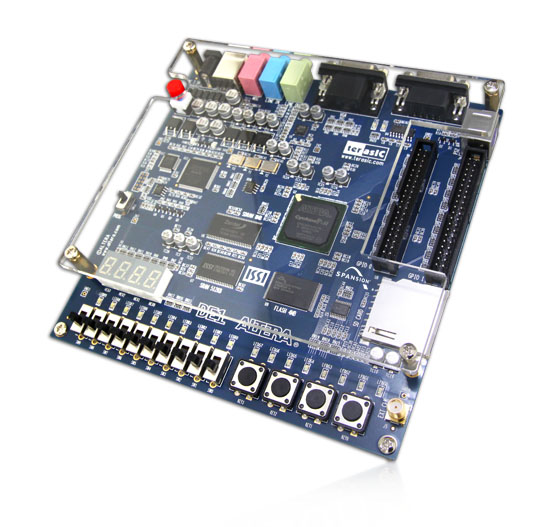
\includegraphics[width=\textwidth]{de1.jpg}
    \end{subfigure}
    ~
    \begin{subfigure}{0.48\textwidth}
        \centering
        \caption{DE2 board\label{fig:de2}}
        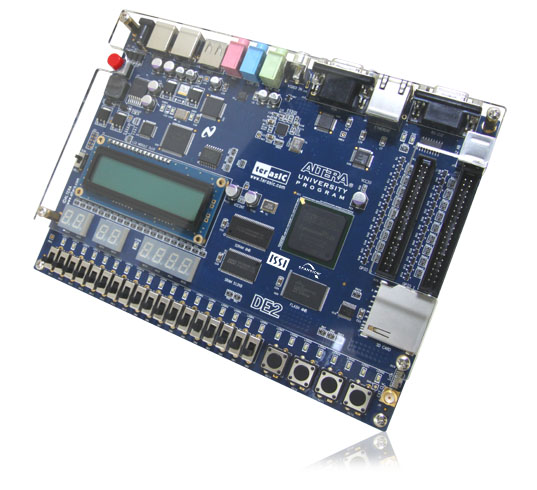
\includegraphics[width=\textwidth]{de2.jpg}
    \end{subfigure}
\end{figure}

\subsection{DE1}

\begin{itemize}
    \item Altera Cyclone~II 2C20 FPGA with 20000 LEs
    \item Altera Serial Configuration devices (EPCS4) for Cyclone~II 2C20
    \item USB Blaster built-in on board for programming and user API controlling
    \item JTAG Mode and AS Mode are supported
    \item \SI{8}{\mega\byte} (1M x 4 x 16) SDRAM
    \item \SI{4}{\mega\byte} Flash Memory
    \item \SI{512}{\kilo\byte} (256Kx16) SRAM
    \item SD Card Socket
    \item 4 Push-button switches
    \item 10 DPDT switches
    \item 8 Green User LEDs
    \item 10 Red User LEDs
    \item 4 Seven-segment LED displays
    \item \SI{50}{\mega\hertz} oscillator, \SI{24}{\mega\hertz} oscillator, \SI{27}{\mega\hertz} oscillator and external clock sources
    \item 24-\SI{}{\bit} CD-Quality Audio CODEC with line-in, line-out, and microphone-in jacks
    \item VGA DAC (4-\SI{}{\bit} R-2R per channel) with VGA out connector
    \item RS-232 Transceiver and 9-pin connector
    \item PS/2 mouse/keyboard connector
    \item Two 40-pin Expansion Headers (GPIO: voltage levels: \SI{3.3}{\volt})
    \item DE1 Lab CD-ROM which contains many examples with source code
\end{itemize}

\subsection{DE2}

\begin{itemize}
    \item Altera Cyclone~II 2C35 FPGA with 35000 LEs
    \item Altera Serial Configuration devices (EPCS16) for Cyclone~II 2C35
    \item USB Blaster built in on board for programming and user API controlling
    \item JTAG Mode and AS Mode are supported
    \item \SI{8}{\mega\byte} (1M x 4 x 16) SDRAM
    \item \SI{512}{\kilo\byte} (256K X16) SRAM
    \item \SI{4}{\mega\byte} Flash Memory (upgradeable to \SI{4}{\mega\byte})
    \item SD Card Socket
    \item 4 Push-button switches
    \item 18 DPDT switches
    \item 9 Green User LEDs
    \item 18 Red User LEDs
    \item 16 x 2 LCD Module
    \item \SI{50}{\mega\hertz} and \SI{27}{\mega\hertz} (from TV decoder) for clock sources
    \item 24-\SI{}{\bit} CD-Quality Audio CODEC with line-in, line-out, and microphone-in jacks
    \item VGA DAC (10-bit high-speed triple DACs) with VGA out connector
    \item TV Decoder (NTSC/PAL) and TV in connector
    \item 10/100 Ethernet Controller with the socket.
    \item USB Host/Slave Controller with USB type A and type B connectors.
    \item RS-232 Transceiver and 9-pin connector
    \item PS/2 mouse/keyboard connector
    \item IrDA transceiver
    \item Two 40-pin Expansion Headers with diode protection
    \item DE2 Lab CD-ROM which contains many examples with source code to exercise the boards, including SDRAM and Flash Controller,  CD-Quality Music Player, VGA and TV Labs, SD Card reader, RS-232/PS-2 Communication Labs, NIOSII, and Control Panel API
\end{itemize}

More information about these boards is provided in their manuals on your desktops. Please refer to the manual for pin assignments. 

\section*{Acknowledgment}
\addcontentsline{toc}{section}{Acknowledgment}

This manual has been revised and edited by \href{mailto:hadi.safari@ut.ac.ir?subject=[DLDLab]\%20}{Hadi Safari}, undergraduate student of Computer Engineering at University of Tehran.

\end{document}
